
\date{\today}
\title{Packet Analysis with Wireshark}


\documentclass[12pt]{article}

\usepackage{graphicx}

\author{
  Singhal, Madhur\\
  \texttt{2015CS10235}
  \and
  Chhajwani, Anant\\
  \texttt{2015CS50281}
}

\begin{document}
\maketitle


\section{Introduction}
Wireshark is a free and open source packet analyzer. It provides a Graphical User Interface for viewing packets that are travelling through the computer. Wireshark also decomposes the packet and extracts the fields for each layer the packet has encapsulated in it.


\paragraph{}
In this Assignment part we first use wireshark to understand different types of packets sent or receieved by our computer. Later we go on to analyze some simple requests and analyze the progression of packets related to them. All these experiments are done on a computer on WiFi running Ubuntu 17.10.

\section{Background Packets}

We captured the background packets for 60 seconds. Below are two pictures showing the different types of Protocols and Destinations that background packets comprise of.

\paragraph{}
\begin{center}
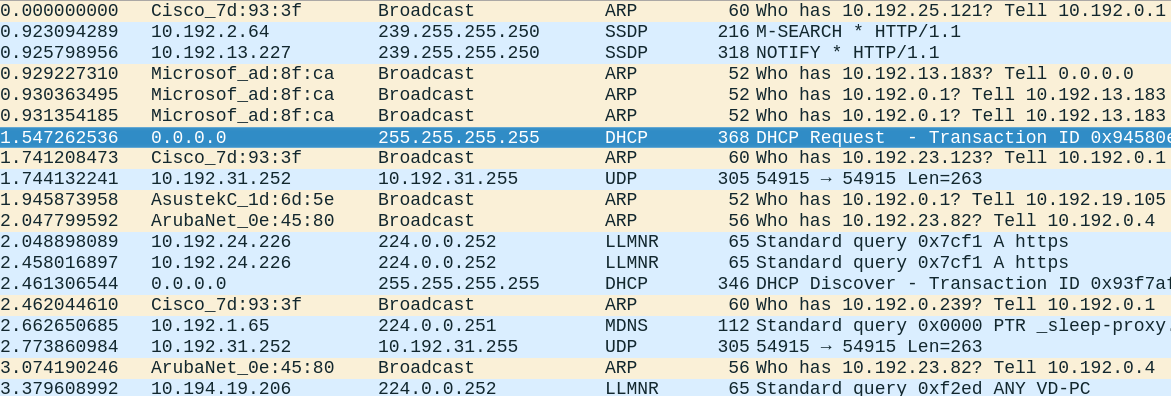
\includegraphics[scale=0.4]{f3}
.
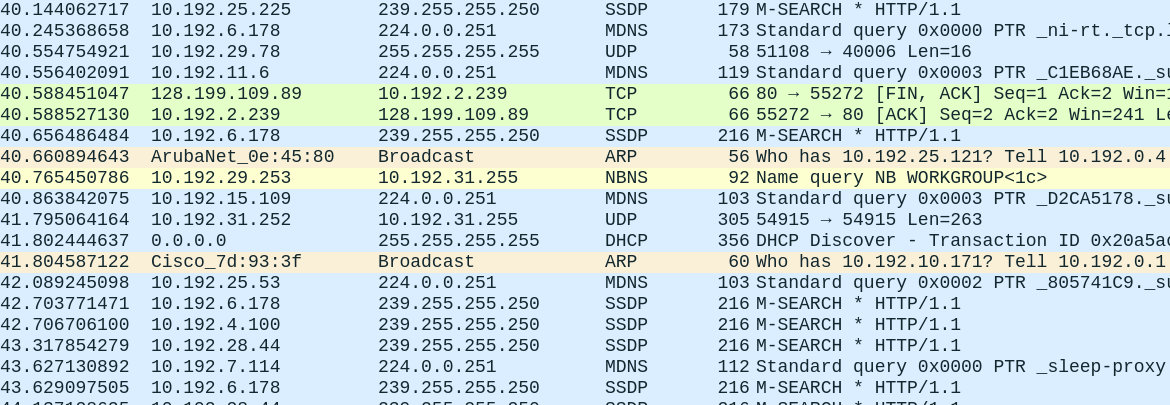
\includegraphics[scale=0.4]{f4}

\end{center}

\paragraph{Applications}

\begin{enumerate}
\item \textbf{ARP Packets} The IP module generates the ARP (Address Resolution Protocol) packets. They are used to resolve local IP addresses into MAC addresses. The Destination address for such packets is "Broadcast" which means they are automatically sent to all receivers on the WiFi Network.
\item \textbf{SSDP Packets} The SSDP (Simple Service Discovery Protocol is used to discover services being offered on the local network. The SSDP packets were originating elsewhere so I think the application generating them was in some other computer on the network. Some analysis suggests that windows may be automatically sending those packets to search for services.
\item \textbf{LLMNR Packets} The LLMNR (Link-Local Multicast Name Resolution) is used to resolve addresses to local addresses. It is generated by systemd on Ubuntu.
\item \textbf{MDNS Packets} The MDNS ( Multicast Domain Name System) is used  in this context for providing wake on ping services. Apple devices provide this service, wherein you can wake up a sleeping device by sending a proper packet to it.
\item \textbf{NBNS Packets} The NBNS (Net Bios Name Resolution System) provides name resolution for legacy Net-Bios over IP Services. It is primarily used by Windows to maintain it's sharing features.
\item \textbf{Miscellaneous Packets} There are some other TCP and UDP packets with encrypted data so I can't find out what is generating them. Could be vestiges of previous connections to web servers before starting the scan.
\end{enumerate}

\section{Analysis of Webpage Fetch}


\begin{center}
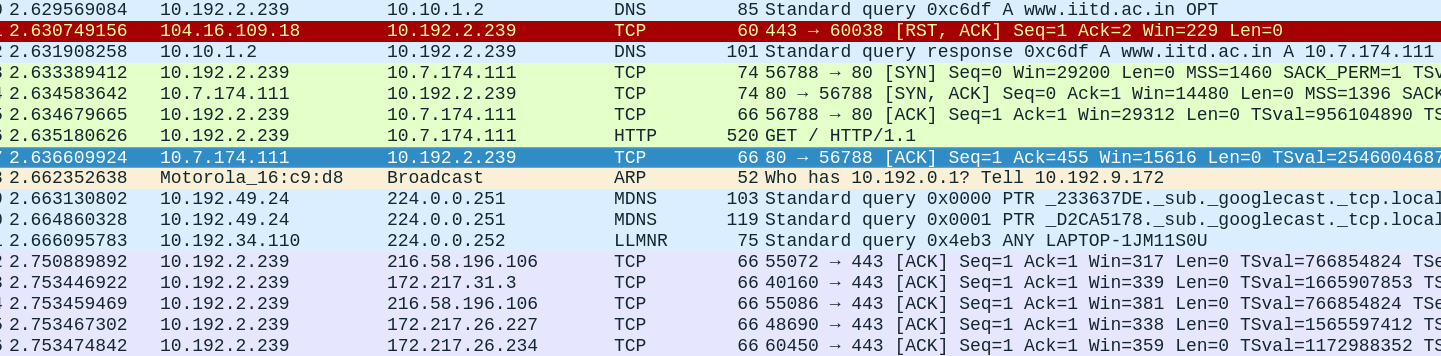
\includegraphics[scale=0.3]{f5}
\end{center}




\begin{enumerate}
\item \textbf{Servers for which a DNS query was launched} Only one DNS query for www.iitd.ac.in was launched. The response was 10.7.174.111. 
\item \textbf{Number of HTTP requests generated} After filtering the packets to http only, I see 162 packets, half of which are requests and the other half are responses. Thus \textbf{81 Requests} are generated.
\item \textbf{Number of TCP connections opened} - 
 \textbf{Six} TCP connections were opened.
\item \textbf{Total time taken for download} The total time taken was \textbf{2.7575 seconds.}
\item \textbf{Any TCP losses/retransmits noticed} No Losses/Retransmits observed.
\end{enumerate}


\begin{figure}[b]
HTTP Request
\begin{center}
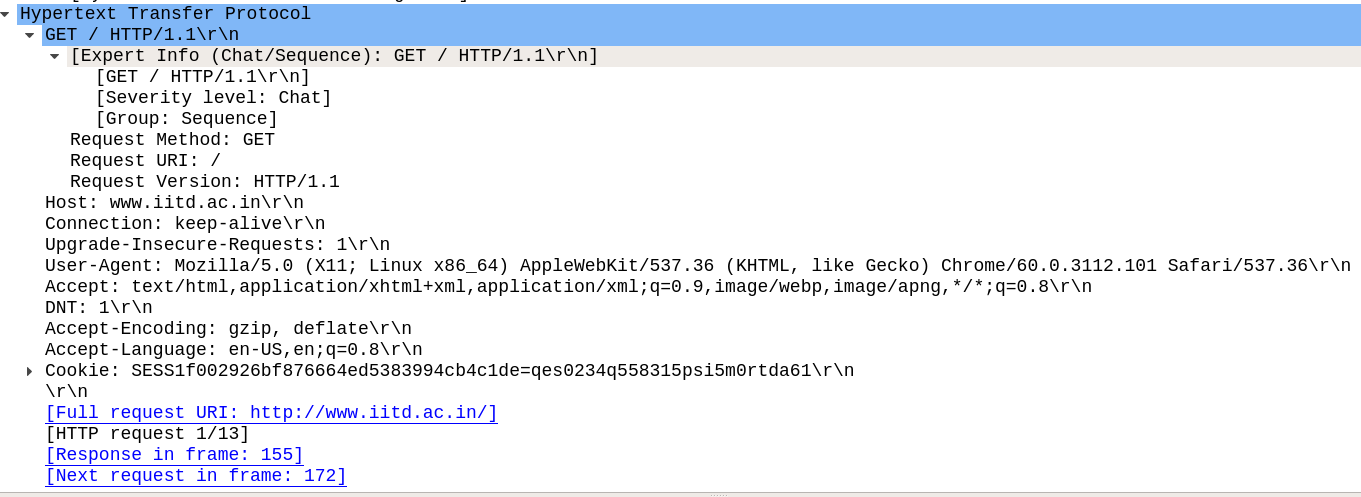
\includegraphics[scale=0.3]{httph}
\end{center}
\end{figure}

\begin{figure}[b]
TCP Header
\begin{center}
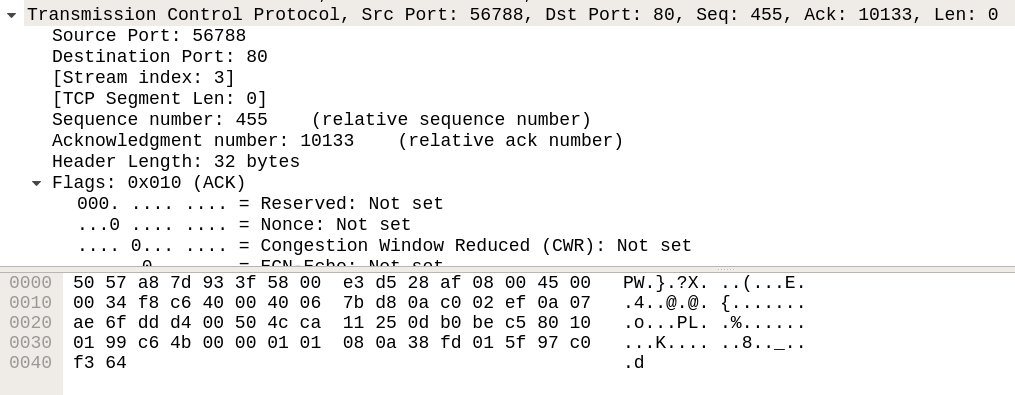
\includegraphics[scale=0.3]{tcph}
\end{center}
\end{figure}

\begin{figure}[b]
IP Header
\begin{center}
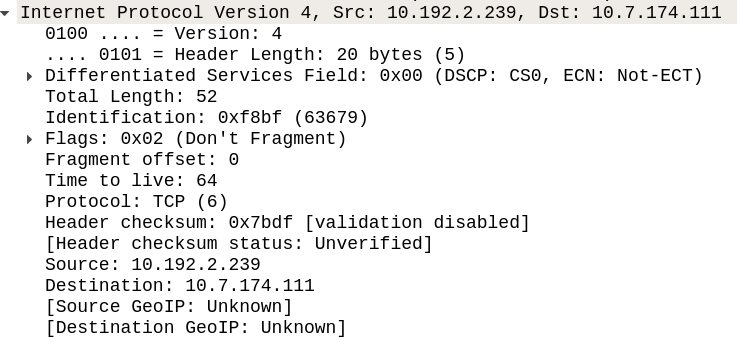
\includegraphics[scale=0.3]{iph}
\end{center}
\end{figure}
\end{document}
